\documentclass[12pt,a4paper]{article}
\usepackage[utf8]{inputenc}
\usepackage[T1]{fontenc}
\usepackage[italian]{babel}

\usepackage{verbatim}

\begin{comment}
\addto\captionsitalian{%
  \renewcommand{\abstractname}{Abstract}%
}
\end{comment}

\usepackage{subcaption}
\usepackage{graphicx}
\usepackage{fancyhdr}
\usepackage{titlesec}
\usepackage{lmodern}
\usepackage{geometry}
\usepackage{setspace}
\usepackage{parskip}
\usepackage{listings}
\usepackage{xcolor}
\usepackage{enumitem}
\usepackage{float}
\usepackage{booktabs}
\usepackage{csquotes}
\usepackage{tabularx} 

\usepackage[
    backend=biber,
    style=numeric,
    sorting=none
]{biblatex}
\addbibresource{bibliography.bib}

\usepackage{hyperref}
\hypersetup{colorlinks=true, linkcolor=blue, citecolor=blue, urlcolor=blue}
\usepackage{xurl}

\addtolength{\skip\footins}{1cm}

\definecolor{codegreen}{rgb}{0,0.6,0}
\definecolor{codeblue}{rgb}{0.2,0.2,0.7}
\definecolor{backcolor}{rgb}{0.95,0.95,0.90}

\lstdefinestyle{mystyle}{
    backgroundcolor=\color{backcolor},   
    commentstyle=\color{codegreen}\itshape,
    keywordstyle=\color{blue},
    numberstyle=\tiny\color{black},
    stringstyle=\color{codegreen},
    basicstyle=\ttfamily\footnotesize,
    breaklines=true,
    captionpos=b,
    keepspaces=true,
    numbers=left,
    numbersep=8pt,
    showspaces=false,
    showstringspaces=false,
    showtabs=false,
    frame=shadowbox,
    language=Python
}

\lstset{style=mystyle}

\geometry{top=2.5cm,bottom=2.5cm,left=2.5cm,right=2.5cm}

% --- CONFIGURAZIONE LISTINGS PER JAVASCRIPT ---
\definecolor{lightgray}{rgb}{.95,.95,.95}
\definecolor{darkgray}{rgb}{.4,.4,.4}
\definecolor{purple}{rgb}{0.65, 0.12, 0.82}

\lstdefinelanguage{JavaScript}{
  keywords={break, case, catch, continue, debugger, default, delete, do, else, false, finally, for, function, if, in, instanceof, new, null, return, switch, this, throw, true, try, typeof, var, void, while, with, const, let},
  morecomment=[l]{//},
  morecomment=[s]{/*}{*/},
  morestring=[b]',
  morestring=[b]",
  ndkeywords={class, export, boolean, throw, implements, import, this},
  keywordstyle=\color{blue}\bfseries,
  ndkeywordstyle=\color{darkgray}\bfseries,
  identifierstyle=\color{black},
  commentstyle=\color{purple}\ttfamily,
  stringstyle=\color{codegreen}\ttfamily,
  sensitive=true
}

\lstdefinelanguage{Dart}{
  keywords={abstract, as, assert, async, await, break, case, catch, class, const, continue, default, deferred, do, dynamic, else, enum, export, extends, extension, external, factory, false, final, finally, for, Function, get, hide, if, implements, import, in, is, late, library, mixin, new, null, on, operator, part, required, rethrow, return, set, show, static, super, switch, sync, this, throw, true, try, typedef, var, void, while, with, yield},
  morecomment=[l]{//},
  morecomment=[s]{/*}{*/},
  morestring=[b]',
  morestring=[b]",
  keywordstyle=\color{blue}\bfseries,
  identifierstyle=\color{black},
  commentstyle=\color{codegreen}\ttfamily,
  stringstyle=\color{codegreen}\ttfamily,
  sensitive=true
}

\lstset{
    style=mystyle,
    language=JavaScript,
    breaklines=true,
    postbreak=\mbox{\textcolor{red}{$\hookrightarrow$}\space},
}


\begin{document}

\begin{titlepage}
    \centering
    \vspace*{1.5cm}
    {\scshape\LARGE Università degli Studi di Udine \par}
    \vspace{0.4cm}
    {\scshape\Large Dipartimento di Scienze Matematiche, Informatiche e Fisiche\par}
    \vspace{0.4cm}
    {\large IBML - Internet of Things, Big Data, Machine Learning \par}
    \vspace{0.4cm}
    \vspace{1.5cm}
    
\includegraphics[width=0.25\textwidth]{immages/logo.pdf}\par
    \vspace{1cm}
    \rule{\textwidth}{0.5pt}\vspace{0.4cm}
    {\bfseries\LARGE Internet of Things\\[0.2cm]
    Progetto Pet Tracker \par}
    \rule{\textwidth}{0.5pt}
    \vfill
    \begin{flushleft}
    \textit{\textbf{Autori}}\\
    Andrea Gioia, 169484 \hfill 169484@spes.uniud.it \\
    Alessio Nicodemo, 166972 \hfill 166972@spes.uniud.it \\
    Mattia Nadal,  167372\hfill 167372@spes.uniud.it \\
    Francesco Sabot, 167339  \hfill 167339@spes.uniud.it
    \end{flushleft}
\end{titlepage}

\begin{abstract}

\noindent 
Il progetto Pet Tracker propone la realizzazione di un sistema 
per il tracciamento in tempo reale di animali domestici di taglia media o grande, 
tramite un dispositivo \textit{embedded} indossabile.
L'obiettivo del lavoro è sviluppare una soluzione affidabile, 
scalabile e a basso consumo per il monitoraggio continuo dell'animale. \\

\noindent
La soluzione si basa su una piattaforma
ESP32-S3 con connettività LTE e modulo GNSS, 
in grado di acquisire e trasmettere 
lo stato della batteria del dispositivo, 
insieme alla posizione geografica e 
all'attività motoria dell'animale, 
verso un \textit{backend} remoto.
L'architettura del sistema segue il modello \textit{IoT World Forum} (IoTWF)
e integra diverse tecniche di ottimizzazione energetica, 
tra cui l'utilizzo delle modalità \textit{deep sleep} e \textit{hot start}. 
I dati raccolti vengono elaborati dal \textit{backend}, resi accessibili tramite API REST 
e visualizzati attraverso un'applicazione mobile dedicata. 

\end{abstract}

\newpage

\tableofcontents

\newpage

\section{Obiettivi del Progetto}

Il progetto Pet Tracker nasce con l'obiettivo generale di realizzare un sistema completo di localizzazione e monitoraggio per animali domestici di taglia media o grande, affidabile, a basso consumo energetico e utilizzabile in scenari reali. Per raggiungere questo obiettivo, il lavoro si è articolato nei seguenti obiettivi specifici:
\begin{itemize}
    \item \textbf{Progettazione hardware del dispositivo indossabile:} integrare su un'unica piattaforma embedded (ESP32-S3) connettività LTE, ricezione GNSS e rilevamento del movimento, garantendo un'autonomia energetica adeguata all'uso continuativo sull'animale.
    \item \textbf{Ottimizzazione energetica del firmware:} implementare strategie di risparmio energetico (\textit{deep sleep}, \textit{hot start}) che permettano di bilanciare la frequenza di acquisizione dei dati con la durata della batteria.
    \item \textbf{Progettazione di un backend affidabile e scalabile:} sviluppare un'infrastruttura server in grado di ricevere, validare e normalizzare i dati grezzi provenienti dal dispositivo, esponendo le informazioni tramite API REST e mantenendo la coerenza storica delle sessioni di attività.
    \item \textbf{Modellazione del comportamento dell'animale:} definire una logica in grado di distinguere in modo affidabile i diversi stati cinematici e geografici dell'animale (permanenza in zona sicura, passeggiata, viaggio in veicolo, allontanamento), riducendo i falsi positivi dovuti al rumore dei sensori.
    \item \textbf{Sviluppo di un sistema di allerta tempestivo:} implementare un meccanismo di notifiche push capace di avvisare l'utente in caso di uscita dal perimetro sicuro o di condizioni critiche del dispositivo, garantendo la gestione di più dispositivi mobili per singolo utente.
    \item \textbf{Realizzazione di un'applicazione mobile intuitiva:} fornire all'utente un'interfaccia in tempo reale per la visualizzazione della posizione, delle statistiche di attività e per la gestione autonoma delle zone di sicurezza, minimizzando il carico sul backend e sui dati mobili.
\end{itemize}

Questi obiettivi guidano la struttura dell'intero elaborato: dopo una panoramica dell'architettura hardware, vengono descritte la logica firmware, il backend e la modellazione dei dati, per poi passare all'applicazione mobile e al sistema di notifiche, fino ai vincoli riscontrati e alle possibili evoluzioni future del sistema.

\clearpage
\section{Hardware}
\label{sec:hardware}

\subsection{LilyGo T-SIM7670G-S3}

Il dispositivo utilizza una scheda LilyGo T-SIM7670G-S3 \cite{lilygo_specs} basata sul microcontrollore ESP32-S3 dual-core.
Quest'ultimo gestisce la logica applicativa e la comunicazione con il modem SIM7670G tramite interfaccia UART.

\subsection{Antenne LTE e GNSS}

Il sistema utilizza un'antenna flessibile LTE \cite{LTE} per la connettività dati e un'antenna ceramica attiva \cite{GPS} per il ricevitore GNSS integrato, garantendo la precisione della localizzazione all'aperto.

\subsection{Batteria e power management}

Il sistema è alimentato da una batteria ricaricabile agli ioni di litio da 3000~mAh e 30~A. Il monitoraggio della carica avviene tramite un partitore di tensione collegato al pin \texttt{ADC\_BAT} (GPIO 4), per calcolarne la percentuale residua.

\subsection{BMA400 e CJMCU-400}

L'accelerometro utilizzato è un BMA400 \cite{bma400} integrato sulla \textit{breakout board} CJMCU-400. Il sensore viene interrogato per rilevare il movimento, consentendo l'implementazione di un contapassi utile al monitoraggio dell'attività motoria dell'animale.

\section{Firmware e logica di funzionamento}

Il firmware, sviluppato in ambiente Arduino per 
il \textit{System on Chip} (SoC) ESP32-S3, 
gestisce l'acquisizione dei dati dai sensori, 
il controllo del modem LTE e l'ottimizzazione energetica 
tramite una macchina a stati finiti.

\subsection{Gestione della persistenza e hot start}

Nel tracciamento satellitare, il \textit{Time To First Fix} (TTFF) 
rappresenta il tempo impiegato dal modulo GNSS, a partire dalla sua accensione, 
per acquisire i dati satellitari e calcolare la prima coordinata valida. 
Trattandosi di un processo che richiede di mantenere il modulo radio attivo a lungo, 
costituisce la fase a maggior consumo.

Per massimizzare la durata della batteria, il dispositivo utilizza il \textit{deep sleep}, 
uno stato di ibernazione in cui l'ESP32 spegne la CPU e la memoria principale. 
L'unico componente che rimane acceso è il modulo \textit{Real-Time Clock} (RTC) dell'ESP32, 
dotato di una piccola memoria dedicata. 
Per ridurre il TTFF, il firmware sfrutta quest'area per preservare i dati critici durante i cicli di \textit{deep sleep}.  
Dove, le variabili come l'ultima posizione valida (\texttt{lastLat}, \texttt{lastLon}) 
e i timestamp (\texttt{lastGpsDate}, \texttt{lastGpsTime}) vengono dichiarate con l'attributo \texttt{RTC\_DATA\_ATTR}, 
permettendo al sistema di ritrovarle intatte al risveglio.

\newpage

Al risveglio del dispositivo, la funzione \texttt{iniettaGps()} esegue le seguenti operazioni:
\begin{itemize}
    \item Recupera le coordinate geografiche e temporali salvate nel ciclo precedente;
    \item Inietta la posizione nota nel modulo GNSS tramite il comando \texttt{AT+CGNSSPOS};
    \item Sincronizza l'orologio interno del modem con il comando \texttt{AT+CGNSSTIME}.
\end{itemize}

Questo meccanismo abilita la modalità \textit{hot start}, 
che permette di agganciare il segnale in pochi secondi, 
abbattendo drasticamente il consumo energetico.

\subsection{Protocollo di comunicazione HTTPS}

La trasmissione dei dati al \textit{backend} PocketBase è affidata a una serie di comandi AT inviati
via seriale al modem SIM7670G. Il firmware incapsula le informazioni in un oggetto JSON
strutturato, trasmesso tramite una richiesta HTTPS POST. Il \textit{payload} include:

\begin{itemize}
    \item \texttt{board\_id}: un identificativo univoco derivato dall'IMEI del modem;
    \item \texttt{geo}: un oggetto con latitudine e longitudine per la localizzazione geografica;
    \item \texttt{battery} / \texttt{battery\_percent} / \texttt{charging}:
          dati sullo stato di carica della batteria;
    \item \texttt{steps}: conteggio dei passi rilevato dall'accelerometro nella sessione corrente;
    \item \texttt{sleep}: flag booleano che segnala al server l'imminente entrata in stato
          di inattività;
    \item \texttt{trip}: flag booleano che segnala al server che l'animale si trova su un
          veicolo in movimento. Quando attivo, ignora le regole del \textit{geofencing}
          e sospende il \textit{deep sleep} per garantire la continuità del tracciamento.
\end{itemize}

La sequenza di invio utilizza i comandi 
\texttt{AT+HTTPINIT} per inizializzare il servizio HTTP del modem, 
\texttt{AT+HTTPPARA} per definire i parametri della connessione,
\texttt{AT+HTTPDATA} per specificare la dimensione del JSON,
e infine \texttt{AT+HTTPACTION=1} per avviare la trasmissione. 
Al termine di ogni invio, \texttt{AT+HTTPTERM} 
chiude la sessione per liberare le risorse del modem.

\subsection{Risparmio energetico}

Per massimizzare l'autonomia, la gestione energetica 
viene modulata in base alla rilevazione del movimento e allo stato di viaggio:

\begin{enumerate}
    \item \textbf{Rilevamento attività:} il firmware monitora costantemente il numero di passi ricevuto ad ogni pacchetto,
          azzerando a ogni nuovo movimento un timer di inattività (\texttt{lastActivityTime}) per monitorare lo stato di anomalia o di chiusura dell'attività in corso.
    \item \textbf{Modalità viaggio:} se il flag \texttt{trip} è attivo (velocità GPS $>$ 10\,km/h), 
          il \textit{deep sleep} viene disabilitato indipendentemente dall'inattività rilevata
          dall'accelerometro, garantendo la trasmissione dei dati a intervalli regolari durante il viaggio.
    \item \textbf{Ibernazione:} se non viene rilevata attività per un tempo superiore a
          \texttt{SLEEP\_TIMEOUT} (30~secondi) e il flag \texttt{trip} non è attivo, il sistema
          invia un ultimo pacchetto dati aggiornando il flag \texttt{sleep} a \texttt{true}, entrando in \textit{deep sleep}. 
          Vengono quindi spenti i moduli radio tramite i comandi \texttt{AT+CGNSSPWR=0} e \texttt{AT+CPOWD=1}. Il risveglio
          è gestito tramite interrupt hardware sul pin \texttt{GPIO\_5}, generato dall'accelerometro
          solo al rilevamento di un nuovo movimento.
\end{enumerate}

Inoltre, il firmware integra specifiche strategie di controllo energetico 
volte a eliminare i consumi statici e a prevenire alterazioni nelle letture dei sensori:

\begin{itemize}
    \item \textbf{Controllo ADC:} il circuito del partitore di tensione per la batteria viene
          attivato solo durante la lettura tramite il pin \texttt{BAT\_ADC\_EN}, garantendo la
          precisione del voltaggio acquisito dal pin \texttt{ADC\_BAT}. Il valore grezzo viene
          mediato su 10 campionamenti consecutivi e scalato con fattore pari a 2 per compensare il partitore. 
          La percentuale di carica è calcolata per interpolazione lineare
          nell'intervallo compreso tra 3,4~V e 4,2~V,
          corrispondenti rispettivamente a 0\% e a 100\% di carica.
    \item \textbf{Stato USB:} dal registro hardware \texttt{USB\_SERIAL\_JTAG\_\allowbreak EP1\_CONF\_REG} dell'ESP32, 
          il sistema rileva se il dispositivo è collegato a una fonte di ricarica USB, impostando
          dinamicamente il campo \texttt{charging} nel pacchetto dati. In stato di ricarica,
          la lettura della batteria viene interrotta per evitare alterazioni dovute alla tensione 
          in ingresso e vengono trasmessi semplicemente gli ultimi dati validi salvati nella memoria RTC.
\end{itemize}

\subsection{Acquisizione GPS e timeout}

Per acquisire la posizione, il firmware interroga il modulo GNSS tramite il comando \texttt{AT+CGNSSINFO}.
La risposta viene analizzata campo per campo, estraendo latitudine, longitudine e velocità in formato decimale. 
Questo evita al microcontrollore il dover decodificare il protocollo standard NMEA, 
che esprime le coordinate in gradi e minuti e richiederebbe calcoli matematici 
aggiuntivi per ricavare il formato decimale utilizzato dalle mappe moderne per il \texttt{backend}.
Il firmware attende fino al \texttt{GPS\_TIMEOUT} (180~secondi) per ottenere
una posizione valida; superato tale limite senza successo, il ciclo corrente viene
saltato e il sistema ritenta al loop successivo. Ottenute invece le coordinate, queste
e il timestamp vengono salvati in memoria RTC per abilitare l'\textit{hot start} al ciclo successivo.

\subsection{Connessione alla rete LTE}

All'avvio, attraverso la funzione \texttt{connectToNetworkFast()},
il firmware tenta di registrarsi alla rete LTE. Vengono configurati la modalità radio
(\texttt{AT+CNMP=38} per LTE), il profilo APN dell'operatore e l'attivazione del
contesto dati con \texttt{AT+CNACT=0,1}. La registrazione viene verificata tramite interrogazioni periodiche
con il comando \texttt{AT+CEREG?}, controllando che il modem restituisca i codici di stato
\texttt{0,1} (registrato in rete home) o \texttt{0,5} (roaming). Se entro il
\texttt{NET\_TIMEOUT} (60~secondi) la registrazione non viene completata, il dispositivo
entra direttamente in \textit{deep sleep} per evitare consumi inutili in assenza di copertura.

\section{Backend e database}

La gestione della persistenza e della modellazione dei dati è basata su PocketBase \cite{pocketbase},
una soluzione open-source strutturata su SQLite scelta per la sua reattività, 
il ridotto consumo di risorse e il supporto di un'interfaccia API RESTful. 
La logica applicativa lato server e l'integrazione dei flussi di dati si sviluppano estendendo 
il nucleo del framework direttamente nel file principale di runtime \texttt{main.pb.js}, 
che gestisce sia gli eventi reattivi, noti come \textit{hooks}, 
sia i servizi temporali pianificati, definiti come \textit{cron jobs}.
Poiché il runtime JavaScript di PocketBase si basa sull'interprete Goja incorporato in Go, 
l'intera esecuzione del codice avviene in modalità \textit{single-threaded}, 
condividendo il medesimo spazio d'esecuzione globale e lo stesso ciclo di eventi del server.

\subsection{Architettura di hosting e affidabilità del sistema}

L'infrastruttura operativa di backend è stata strutturata per garantire disponibilità dei dati, tolleranza ai guasti e monitoraggio continuo durante la fase di prototipazione e test:
\begin{itemize}
    \item \textbf{Esposizione in rete:} il server PocketBase è ospitato su una \textit{workstation} locale. Data la necessità di connettersi al backend sia dal dispositivo (tramite rete cellulare LTE) sia dall'applicazione mobile (tramite rete dati/Wi-Fi), le restrizioni imposte dal NAT e l'assenza di un IP pubblico statico sono state superate mediante l'impiego di ngrok \cite{ngrok}. Questa tecnologia di \textit{tunneling} crea un canale sicuro HTTPS fungendo da \textit{reverse proxy}, reindirizzando il traffico in ingresso verso l'ambiente locale e garantendo l'accessibilità dei servizi in tempo reale.
    \item \textbf{Strategia di backup:} per garantire la resilienza dei dati e prevenire perdite accidentali dovute a guasti del server locale, è stato strutturato un sistema di backup automatizzato tramite rclone \cite{rclone}, uno strumento a riga di comando per la gestione del cloud storage. Il processo è configurato per eseguire la sincronizzazione incrementale della directory dei dati di PocketBase verso un \textit{bucket remoto} su Backblaze B2 \cite{backblaze}, attivato tramite un \textit{cron job} a cadenza mensile.    
    \item \textbf{Monitoraggio esterno:} l'accessibilità e lo stato di salute del sistema sono monitorati esternamente tramite UptimeRobot \cite{uptimerobot}. Poiché l'accessibilità del backend dipende dalla stabilità del tunnel ngrok, il servizio interroga l'endpoint HTTPS a intervalli regolari. Questo permette di rilevare tempestivamente eventuali anomalie di rete, inviando notifiche immediate in caso di interruzione del tunnel o spegnimento del server locale.
\end{itemize}

\subsection{Modellazione dei dati e API rules}

I dati inviati dal dispositivo transitano inizialmente nella collezione di staging \path{data\_sent\_raw}, 
fungendo da \textit{buffer} iniziale per i dati non ancora elaborati, separando la fase di ricezione dalla successiva validazione. 
Il singolo record è strutturato secondo i seguenti campi:

\begin{itemize}
    \item \texttt{timestamp}: riferimento temporale hardware dell'acquisizione;
    \item \texttt{lat} / \texttt{lon}: coordinate geografiche acquisite dal modulo GNSS;
    \item \texttt{battery} / \texttt{battery\_percent}: stato di carica dell'accumulatore espresso in voltaggio e percentuale;
    \item \texttt{charging}: variabile booleana indicante se la batteria è in corso di ricarica;
    \item \texttt{steps}: conteggio lineare dei passi rilevato dall'accelerometro;
    \item \texttt{sleep}: flag booleano indicante se il dispositivo è in stato di \textit{deep sleep};
    \item \texttt{trip}: flag booleano indicante se l'animale si trova su un veicolo in movimento.
\end{itemize}

L'accesso ai dati avviene esclusivamente tramite le API RESTful esposte da PocketBase. 
In questo modo il database rimane totalmente indipendente dall'applicazione mobile sviluppata in Flutter, 
che si limita a richiamare le API per visualizzare i dati.

\begin{comment}
L'integrità e la riservatezza delle informazioni sono rigidamente normate da \textbf{API Rules} basate su espressioni booleane che implementano il principio del minimo privilegio:
\begin{itemize}
    \item \textbf{List/View:} Visualizzazione e interrogazione dei record permesse esclusivamente agli utenti client preventivamente autenticati.
    \item \textbf{Create:} Abilitata per la board LilyGo tramite un account di autenticazione dedicato al dispositivo edge.
    \item \textbf{Update/Delete:} Operazioni distruttive o di modifica strutturale ristrette ai soli amministratori del sistema (\textit{Admin Only}).
\end{itemize}
\end{comment}

\subsection{Pulizia e normalizzazione (Server-side Hooks)}

L'elaborazione dei messaggi IoT segue un pattern architetturale di \textit{Staging-and-Purge} 
gestito lato server tramite i \textit{JavaScript Event Hooks} nativi del sistema. 
L'hook \path{onRecordAfterCreateSuccess} si attiva immediatamente dopo il corretto inserimento
di ogni pacchetto grezzo nella collezione \texttt{data\_sent\_raw}. 
Per ottimizzare le prestazioni ed eliminare letture ridondanti,
il sistema effettua un unico accesso iniziale per recuperare la configurazione del dispositivo (\texttt{getBoardRecord}) 
all'inizio dell'esecuzione dell'hook, distribuendo il record ottenuto come parametro a tutte le funzioni della pipeline. 
L'intero flusso di elaborazione si articola in quattro fasi sequenziali:

\begin{enumerate}
    \item \textbf{Batteria:} salva il record in una collezione dedicata \texttt{battery\_data} e verifica se inviare notifiche push per segnalare livelli critici di batteria.
    \item \textbf{Activity Tracking:} delega l'analisi della telemetria al modulo \path{activity\_manager.js}, che aggiorna la macchina a stati e gestisce la persistenza delle sessioni.
    \item \textbf{Posizioni:} salva le coordinate GPS nella collezione \texttt{positions}, associandole all'attività identificata al punto precedente, a condizione che i dati GNSS risultino attendibili e l'attività sia considerata valida.
    \item \textbf{Eliminazione dato grezzo:} rimuove permanentemente il record originario da \texttt{data\_sent\_raw} all'interno del blocco \texttt{finally} dell'hook. Questo costrutto non serve a garantire l'atomicità transazionale (poiché l'evento scatta a inserimento già avvenuto), ma funge da meccanismo di sicurezza per l'ottimizzazione dello spazio. Infatti, assicura la cancellazione fisica del record di staging e previene la crescita incontrollata del database SQLite, anche qualora una delle funzioni precedenti della pipeline dovesse lanciare un'eccezione non gestita a runtime.
\end{enumerate}

\subsection{Macchina a stati delle attività}

Il modulo \texttt{activity\_manager.js} implementa una macchina a stati 
che classifica il movimento e la posizione dell'animale, 
in funzione dell'area di \textbf{geofence}, dell'\textbf{allarme} impostato dall'utente 
e della \textbf{velocità} dell'animale.
Ogni stato operativo assume una diversa nomenclatura e conserva lo stesso significato logico, 
a seconda che il dispositivo sia \textit{attivo} o in \textit{sleep} (\textit{deep sleep}), 
mantenendo una corrispondenza biunivoca riassunta nella Tabella~\ref{tab:stati}.

\begin{table}[H]
\centering
\small
\begin{tabularx}{\textwidth}{m{2.3cm}m{2.1cm}ccX}
\toprule
\textbf{Attivo} & \textbf{Sleep} & \textbf{Allarme} & \textbf{Geofence} & \textbf{Descrizione posizione}                   \\ \midrule
\texttt{i} (inside)   & \texttt{d}           & True/False              & True              & All'interno dell'area sicura. \\
\texttt{v} (trip)  & \texttt{a}           & False                   & False             & In viaggio su veicolo.        \\ 
\texttt{r} (trip)   & \texttt{q}           & True                    & False             & Rischio di furto su veicolo.  \\
\texttt{w} (walk)     & \texttt{z}           & False                   & False             & In passeggiata.               \\
\texttt{s} (search)   & \texttt{p}           & True                    & False             & Rischio di fuga.              \\ \bottomrule
\end{tabularx}
\caption{stati di posizionamento dell'animale.}
\label{tab:stati}
\end{table}

A livello di archiviazione, l'ingresso in uno stato di sleep chiude la sessione corrente, 
impostando il flag \texttt{is\_active = false}. 
Tuttavia, al momento di elaborare i nuovi dati, il sistema ha bisogno di recuperare il contesto originario dell'animale. 
Per questo motivo, prima di applicare la logica di classificazione, la funzione \texttt{computeStatus} 
normalizza internamente lo stato di sleep, riconducendolo al suo equivalente attivo 
tramite il dizionario \texttt{SLEEP\_TO\_ACTIVE} (es. \texttt{"d"} $\rightarrow$ \texttt{"i"}). 
Questo meccanismo garantisce la continuità dell'analisi anche dopo lunghe fasi di inattività hardware. 

Per evitare la frammentazione dei dati e ottimizzare le query storiche, 
il sistema applica un principio di \textbf{continuità temporale}.
Finché l'animale permane nel medesimo stato, 
il sistema non crea nuovi record nel database, 
ma si limita ad aggiornare il timestamp finale (\texttt{end\_time})
e a incrementare il conteggio dei passi (\texttt{total\_steps}). 
L'inserimento di una nuova riga nel database, con la contestuale chiusura della precedente,
avviene esclusivamente in presenza di un'effettiva transizione di stato. 
Una transizione tra \texttt{"v"} e \texttt{"r"}, indotta dal cambio manuale del flag di allarme
da parte dell'utente, forza la chiusura e la riapertura immediata della sessione, 
permettendo di storicizzare l'evento e di adeguare istantaneamente la priorità delle notifiche.
Le transizioni tra gli stati sono governate da un algoritmo a priorità decrescente:

\begin{enumerate}
    \item \textbf{Priorità 1 (massima):} se il sensore rileva che l'animale è in viaggio (\texttt{trip = true}) e il contatore dei passi è nullo (\texttt{steps == 0}), lo stato viene forzato a \texttt{"v"} o \texttt{"r"} in base all'allarme. Questa condizione funge da filtro per i falsi positivi, ignorando eventuali vibrazioni o rumori dell'accelerometro.
    \item \textbf{Priorità 2:} se l'animale non è in viaggio (\texttt{trip = false}) ma non sono stati ancora rilevati passi (\texttt{steps == 0}), il sistema applica una memoria di stato. Nel dettaglio, assume che il veicolo sia momentaneamente fermo (es. a un semaforo o in sosta con l'animale a bordo) e preserva lo stato \texttt{"v"} o \texttt{"r"} corrente. Il ricalcolo della posizione si attiva solo se \texttt{steps > 0}, ovvero al primo movimento dell'animale.
    \item \textbf{Priorità 3:} se l'animale è nell'area di geofence, lo stato viene impostato a \texttt{"i"}.
    \item \textbf{Priorità 4 (minima):} se l'animale si trova all'esterno dell'area sicura, il sistema valuta il \textit{flag} di allarme per determinare lo stato finale, impostando \texttt{"w"} (passeggiata) in caso di allarme disattivato, oppure \texttt{"s"} (ricerca) in caso di allarme attivato.
\end{enumerate}

\subsection{Lifecycle del deep sleep e servizi temporali}

\subsubsection{Gestione del risveglio e ripristino dello stato}

Al termine di un ciclo di \textit{deep sleep}, il dispositivo riprende le trasmissioni inviando un nuovo pacchetto dati. 
In quel momento non è presente alcuna sessione attiva sul database, 
poiché quest'ultima viene forzatamente chiusa al passaggio in modalità a basso consumo.
Per garantire la continuità logica, il sistema interroga lo storico escludendo eventuali 
record anomali e recupera l'ultima sessione valida archiviata (\texttt{recentClosed}). 
Questo passaggio è fondamentale per estrarre lo stato precedente (\texttt{prevStatus}), 
parametro necessario per la corretta esecuzione della funzione \texttt{computeStatus},
che gestisce il risveglio secondo due scenari:
\begin{itemize}
    \item \textbf{Risveglio nello stesso stato:} si verifica quando lo stato rilevato al risveglio coincide con l'equivalente \textit{attivo} dell'ultimo stato di \textit{sleep}. Ad esempio, se il dispositivo si era sospeso in area sicura (stato \texttt{d}, equivalente a \texttt{i}) e al risveglio rileva che il nuovo stato è ancora \texttt{i}, la sessione pregressa viene semplicemente riaperta (\texttt{is\_active = true}). Questo approccio evita la frammentazione dei record, unificando le attività separate dalla fase di sospensione.
    \item \textbf{Risveglio con cambio di stato:} si verifica quando il nuovo stato rilevato non coincide con l'equivalente \textit{attivo} del precedente stato di \textit{sleep}. In questo caso, il sistema separa nettamente le due fasi, storicizza definitivamente la sessione pregressa, normalizzandone lo stato nella rispettiva controparte \textit{attiva} (es. lo stato \texttt{d} viene convertito in \texttt{i}) per garantire la coerenza storica. Subito dopo, istanzia un nuovo record nel database per il nuovo stato. 
\end{itemize}

Per ottimizzare l'efficienza del thread unico di esecuzione, il modulo implementa 
un \textbf{filtraggio delle notifiche spurie}: 
se viene ricevuto un pacchetto con "\texttt{sleep = true}" in assenza di una sessione attiva sul database, 
l'inserimento viene intercettato e scartato preventivamente a livello logico, 
impedendo la proliferazione di record ridondanti e l'invio di catene di notifiche push duplicate all'utente.

\subsubsection{Watchdog e split notturno}

La coerenza temporale delle sessioni di attività e l'allineamento dello storico sono garantiti da due \textit{cron job}, registrati all'avvio all'interno del \textit{thread} principale dell'applicazione:
\begin{itemize}
    \item \textbf{Watchdog:} ogni minuto interroga il database, per individuare e interrompere le sessioni attive da cui non si ricevono aggiornamenti per oltre 10 minuti, tipicamente a seguito di malfunzionamenti o perdite di connettività LTE. Per preservare lo storico, il modulo chiude forzatamente il record (\texttt{is\_active = false}), lo marca come anomalo (\texttt{anomaly = true}) e notifica tempestivamente l'utente. Da questa procedura di sicurezza sono escluse per \textit{design} le attività in \textit{sleep}, la cui inattività prolungata rientra nel normale funzionamento.    
    \item \textbf{Split notturno:} suddivide le sessioni operative che si protraggono a cavallo di due giornate (esattamente alle 23:59 ora italiana), al fine di non alterare le statistiche grafiche giornaliere visibili all'utente. Poiché i \textit{timestamp} sono memorizzati nativamente da pocketbase in UTC, il sistema gestisce dinamicamente l'alternanza tra ora solare (CET, 22:59:59 UTC) e ora legale (CEST, 21:59:59 UTC) tramite la funzione \texttt{getItalyTime()}, evitando l'impiego di valori di fuso orario statici. Il \textit{cron job} è pertanto schedulato per avviarsi in entrambi i possibili orari critici. Sarà poi un controllo interno, basato sul fuso orario attivo, a bloccare l'esecuzione nel caso in cui l'orario non corrisponda a quello effettivo. In fase di elaborazione, le sessioni in stato di \textit{sleep} vengono preventivamente riattivate per garantire l'integrità dello storico, mentre le occorrenze già marcate come anomale (\texttt{anomaly = true}) vengono ignorate, impedendone la duplicazione nel giorno successivo.
\end{itemize}

\section{Frontend e applicazione mobile}

L'applicazione mobile è stata sviluppata 
in \textit{Flutter} \cite{flutter}, un framework
cross-platform che consente di produrre un'unica 
base di codice per Android e iOS.
I test sono stati condotti \textbf{esclusivamente su 
ambiente Android} a causa di vincoli tecnici. 
Nello specifico, l'assenza di postazioni di lavoro con macOS 
ha impedito la compilazione per l'ecosistema Apple, 
a cui si aggiunge la mancanza di una licenza per l'\textit{Apple Developer Program}, 
necessaria per superare il limite di persistenza 
di sette giorni previsto per i profili gratuiti su dispositivo fisico.
La comunicazione con il backend avviene tramite 
il PocketBase SDK ufficiale per \texttt{Dart}, 
che gestisce le chiamate REST e i meccanismi di autenticazione.

\subsection{Architettura a livelli}

Il codice è strutturato in quattro livelli principali, per separare le diverse responsabilità:

\begin{itemize}
  \item \textbf{Repositories}: accesso ai dati remoti tramite PocketBase SDK,
    fornendo alle schermate dati in tempo reale e pronti all'uso.
  \item \textbf{Models}: definiscono la struttura dei dati 
    convertendo i record JSON del backend in oggetti Dart.
  \item \textbf{Services}: gestiscono le funzionalità di sistema e le integrazioni esterne 
    (autenticazione, mappe, tracciamento GPS e notifiche).
  \item \textbf{Screens}: interfaccia utente che si limita a richiedere i dati ai
    repository e a reagire ai loro aggiornamenti.
\end{itemize}

Questa struttura garantisce un codice ordinato e facile da aggiornare, 
mantenendo la logica di funzionamento ben separata dall'interfaccia grafica.

\subsection{Autenticazione e persistenza della sessione}

Per permettere all'utente di restare collegato in modo permanente e sicuro,
abbiamo esteso l'\texttt{AuthStore} nativo di PocketBase, 
che normalmente salva i dati solo temporaneamente in memoria. 
L'autenticazione è quindi gestita tramite un \texttt{SecureAuthStore} personalizzato 
che agisce come una \textit{cassaforte digitale}, riceve il token (JSON Web Token) 
dal server al momento del login e lo archivia in forma cifrata 
all'interno del dispositivo tramite \texttt{flutter\_secure\_storage}. 
Questo sistema sfrutta i sistemi di protezione hardware del dispositivo 
(Keystore su Android e Keychain su iOS) per impedire accessi non autorizzati.

Al riavvio dell'app, il token viene riletto dallo storage sicuro e viene
tentato un refresh automatico della sessione. In caso di successo, l'utente accede
direttamente alla schermata principale senza dover reinserire le credenziali; in caso di
token scaduto o non valido, lo store viene svuotato e l'utente viene reindirizzato alla schermata di login.

\subsection{Splash screen e caricamento parallelo}

La schermata di avvio svolge un ruolo attivo nel precaricare i dati 
necessari alla home page. Una volta verificata l'autenticazione, 
vengono avviate in parallelo, le seguenti operazioni:

\begin{itemize}
  \item recupero del profilo utente e dello stato dell'allarme;
  \item recupero dell'ultima posizione GPS registrata dal dispositivo;
  \item recupero delle attività del giorno corrente filtrate per \texttt{board\_id}.
\end{itemize}

Il \texttt{board\_id}, identificativo univoco della board LilyGo associata a un dispositivo per utente,
viene risolto dinamicamente interrogando la collezione \texttt{boards} sul backend tramite repository.
Questo permette all'app di trovare il dispositivo corretto automaticamente, 
evitando di dover inserire il codice manualmente nel software.


\subsection{Comunicazione in tempo reale}

Completata la fase iniziale di caricamento dati, l'app stabilisce una 
\textbf{connessione persistente} al database, passando da una visualizzazione 
statica ad un monitoraggio dinamico.

Per le funzionalità che richiedono aggiornamenti continui come la posizione GPS, 
l'app sfrutta il meccanismo di \textit{subscribe} offerto da PocketBase, 
basato su \texttt{Server-Sent Events}. 
I repository (come \texttt{PositionsRepository}) espongono uno \texttt{Stream} tipizzato 
(ad esempio \texttt{Stream<Positions>}) a cui le schermate si sottoscrivono 
tramite una \texttt{StreamSubscription}.

In questo modo, ogni nuovo record inserito nel database viene notificato 
istantaneamente all'app. L'interfaccia utente si aggiorna dinamicamente 
evitando la tecnica del \textit{polling}, che costringerebbe l'app a inviare 
continue richieste al server, ed eliminando la necessità di qualsiasi ricaricamento 
manuale della pagina da parte dell'utente.

Per garantire l'efficienza dell'applicativo e prevenire \textit{memory leak}, 
ogni sottoscrizione viene rigorosamente interrotta tramite il comando
\texttt{cancel()} nel metodo \texttt{dispose()} quando l'utente naviga verso un'altra schermata. 
Questa accortezza evita di mantenere attive connessioni inutili in background, 
ottimizzando l'uso della batteria e del traffico dati.

\subsection{Geofencing e geocoding}

La logica di geofencing è implementata anche dal lato client tramite algoritmo \mbox{\textit{Ray-Casting}}. 
Dato un punto GPS e un poligono definito da una lista di vertici, l'algoritmo traccia un raggio orizzontale dal punto
verso l'infinito e conta le intersezioni con i lati del poligono, se il numero è dispari
indica che il punto è interno al poligono, altrimenti è esterno. 
Questa implementazione sul dispositivo evita un sovraccarico di rete verso il server 
e permette di gestire le funzionalità visive in tempo reale, in totale autonomia dal \textit{backend}.

Le zone vengono recuperate dalla collezione \texttt{geofences} su PocketBase, dove
ogni record memorizza il nome della zona, i dati dell'indirizzo e la lista dei vertici
del poligono. Solo le zone con il flag \texttt{is\_active} impostato a \texttt{true}
vengono considerate nel calcolo. Il risultato della verifica è una stringa con il nome
della zona di appartenenza, oppure \textit{``Fuori zona sicura''} se il punto non
rientra in nessuna area attiva. 

L'app integra un servizio di \textbf{geocoding} 
basato sulle API di \textit{Nominatim} \cite{nominatim},
un motore di ricerca che interroga il database geografico 
open-source di OpenStreetMap per consentire:
\begin{itemize}
  \item \textbf{Reverse Geocoding}: tradurre le coordinate GPS in un indirizzo testuale completo 
  (Via, Civico, CAP e Città) per facilitare la lettura all'utente;
  \item \textbf{Forward Geocoding}: consentire all'utente di creare nuove zone inserendo 
  un indirizzo testuale, che il sistema converte automaticamente in coordinate geografiche 
  per posizionare correttamente il poligono sulla mappa.
\end{itemize}

\subsection{Schermate e funzionalità principali}

\subsubsection{Analisi delle attività}

L’architettura dell’applicazione ruota attorno alla dashboard principale in \texttt{home.dart}, 
che funge da centro di controllo dinamico per il monitoraggio dell'animale, 
mostrandone l'ultima posizione rilevata.
Un'altra caratteristica importante della pagina è l'interruttore dell'allarme.
Se il sistema rileva che l'animale è in stato di fuga, 
l'interfaccia attiva automaticamente un blocco di sicurezza 
per impedirne la disattivazione.
Inoltre, poiché lo stato dell'allarme si basa sulla variabile condivisa \texttt{\_isUpdatingAlarm}, 
l'integrità dell'operazione è garantita da un \textbf{mutex} 
che disabilita temporaneamente l'interruttore durante la sincronizzazione asincrona con il database.
Infine, la schermata raccoglie le statistiche quotidiane 
come passi, chilometri e tempo di attività dell'animale, 
permettendo la consultazione dei dati storici tramite un selettore di data.

La visualizzazione dei dettagli delle attività di una giornata prosegue in 
\texttt{daily\_recap.dart}, che raccoglie e organizza 
in ordine cronologico ogni monitoraggio visualizzato nella dashboard, 
con la possibilità di filtrare per specifiche attività.
Selezionando una determinata sessione dal riepilogo, 
si accede alla schermata \texttt{activity\_details.dart}, 
che mostra il tracciato specifico del percorso tramite una scia continua sulla mappa. 
Il sistema utilizza la funzione \texttt{CameraFit} per centrare l’inquadratura all’apertura, 
garantendo l’immediata visibilità dell’intero tragitto. 
Inoltre, la schermata ripropone le statistiche di passi, chilometri e durata, 
ricalcolate specificamente per l’attività selezionata.

\begin{figure}[htbp]
    \centering
    % Prima immagine (Sinistra)
    \begin{subfigure}[b]{0.47\textwidth}
        \centering
        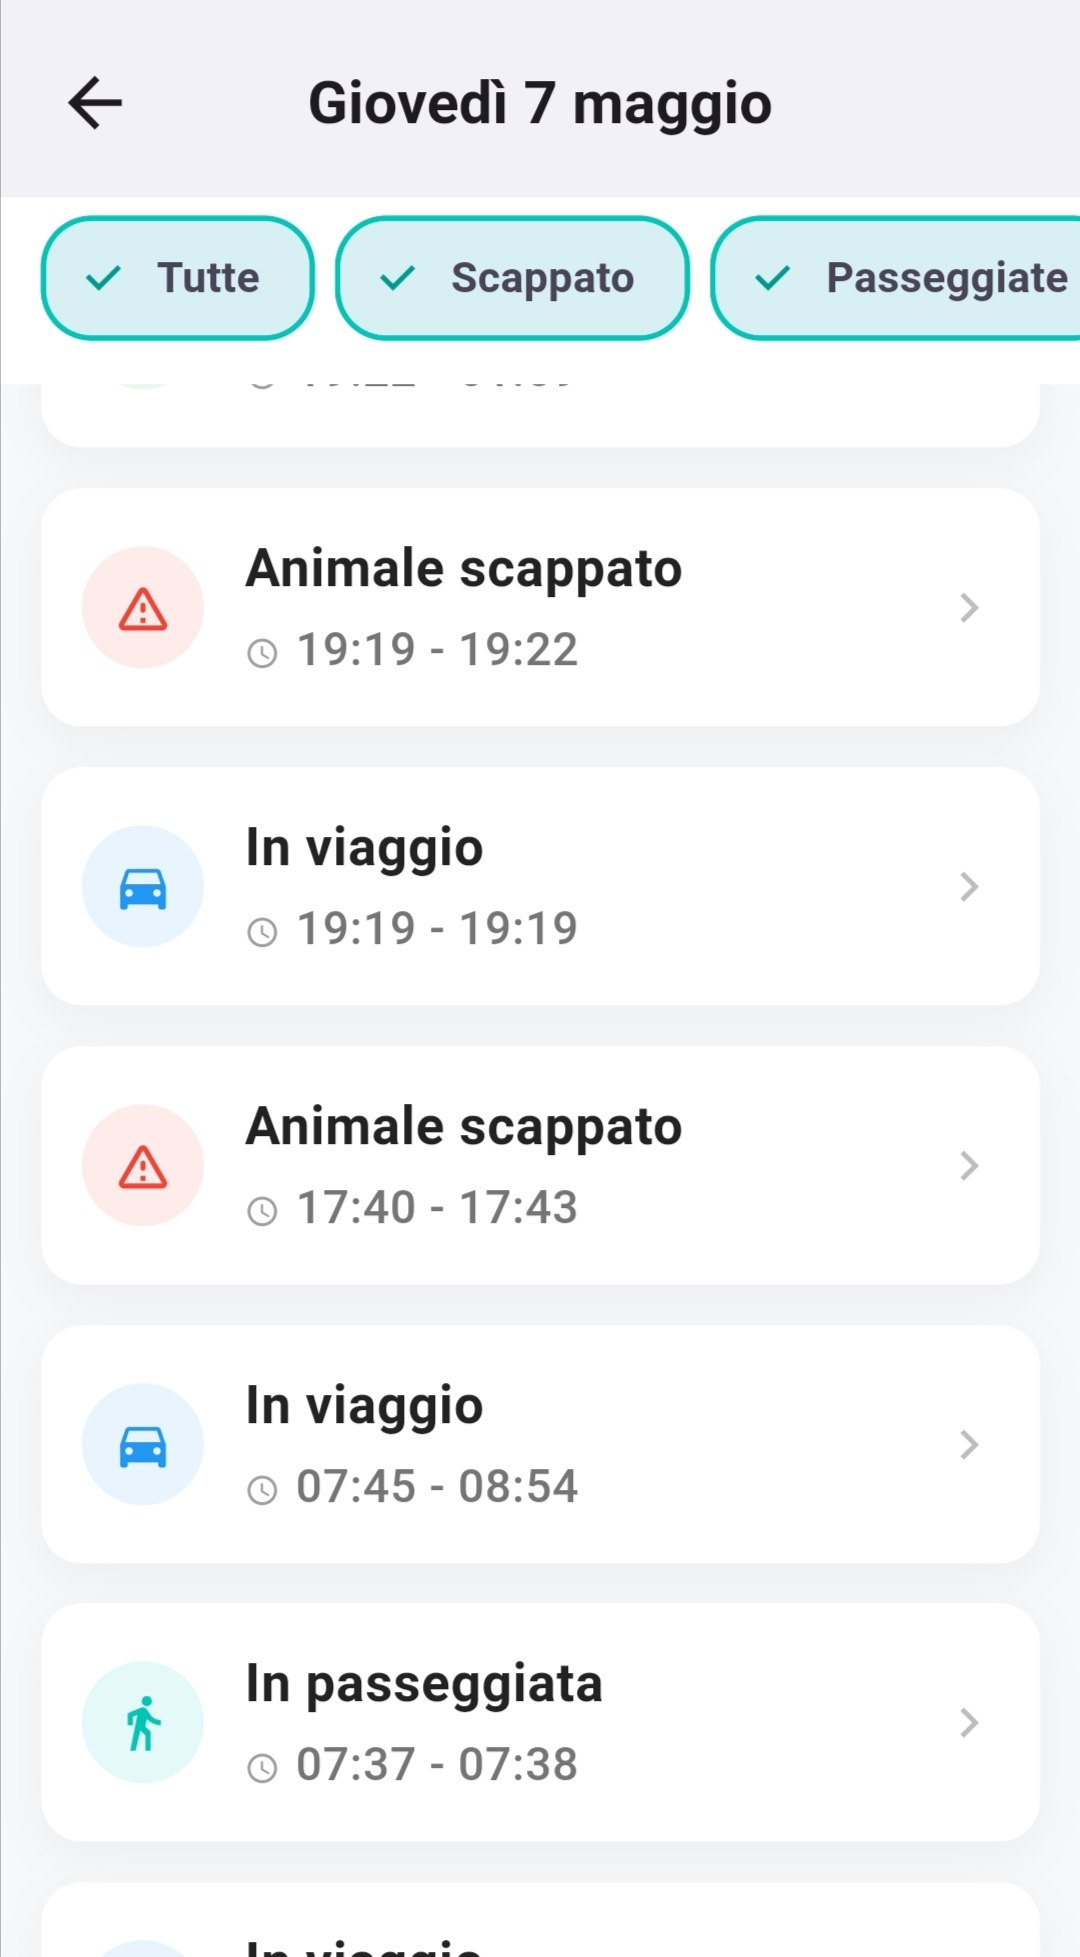
\includegraphics[width=\textwidth, height=8cm, keepaspectratio]{immages/section_5/photo_6.jpg}
        \caption{Visualizzazione di tutte le attività.}
        \label{fig:activity_list}
    \end{subfigure}
    \hfill 
    % Seconda immagine (Destra)
    \begin{subfigure}[b]{0.47\textwidth}
        \centering
        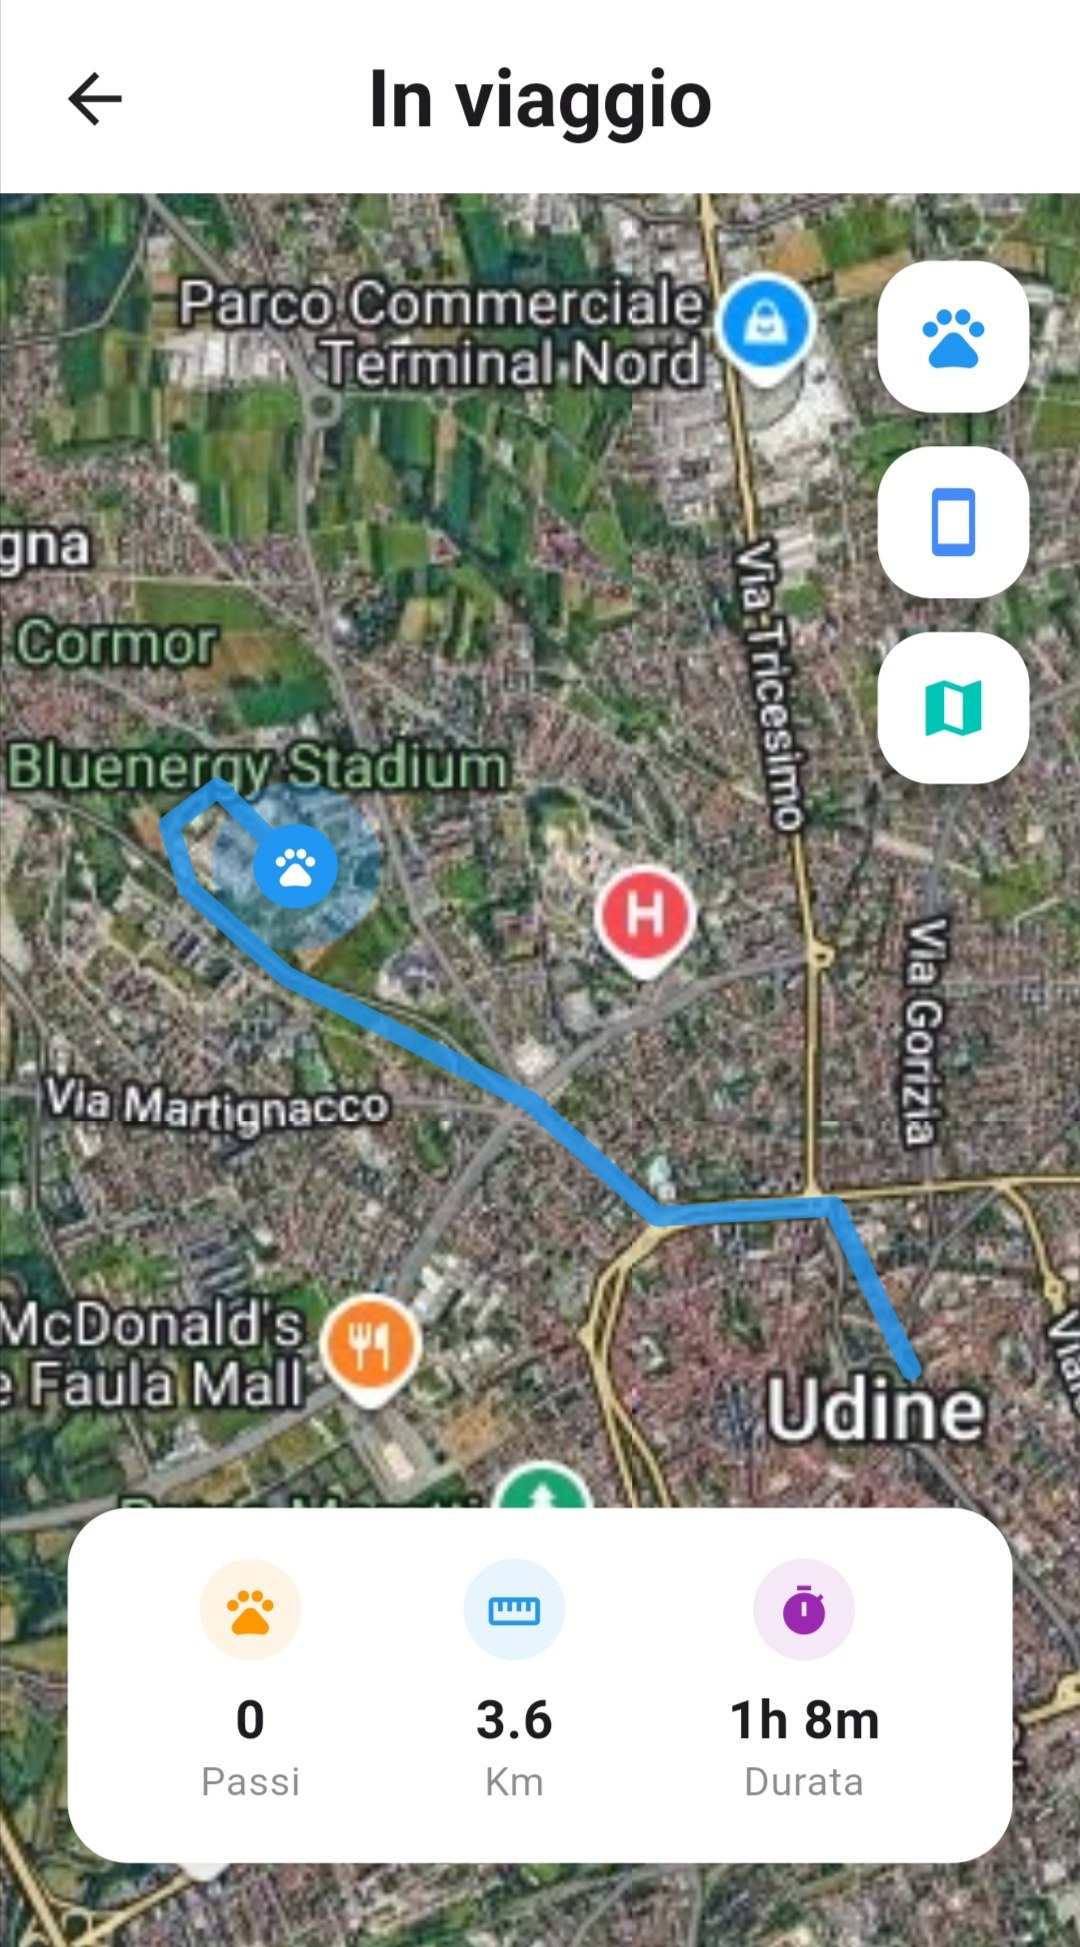
\includegraphics[width=\textwidth, height=8cm, keepaspectratio]{immages/section_5/photo_3.jpg}
        \caption{Dettagli di un'attività.}
        \label{fig:a_form}
    \end{subfigure}
\end{figure}

\subsubsection{Mappe in tempo reale}

L’app utilizza mappe interattive sviluppate con \texttt{flutter\_map}, 
permettendo di localizzare utente e animale in una visuale satellitare o stradale. 
La libreria viene ottimizzata tramite l'uso dei tile di \texttt{OpenStreetMap}, 
ovvero piccoli tasselli d'immagine caricati dinamicamente solo per l'area inquadrata, 
riducendo drasticamente il consumo di dati. 
Per preservare la batteria dello smartphone, 
le posizioni si aggiornano in tempo reale solo quando c'è un vero movimento, 
inoltre l'utente viene localizzato solo se ha dato il permesso.

Il sistema di controllo geografico si articola in due schermate principali 
che si scambiano dinamicamente in base allo stato dell'allarme. 
Quando l'allarme è disattivato, l'utente accede al sistema di \texttt{geofencing.dart}, 
un robusto strumento di sicurezza preventiva che permette di definire e gestire
i confini virtuali rappresentati come poligoni sulla mappa. 

All'attivazione dell'allarme, la schermata \texttt{geofencing.dart} passa a \texttt{tracking.dart}. 
In questa fase, il sistema adotta un approccio proattivo di sicurezza 
implementando un'interfaccia adattiva che cambia tra una modalità 
di monitoraggio e una di "inseguimento" qualora l’animale lasci la sua zona sicura attiva. 
Sulla mappa inoltre viene renderizzata una scia storica 
delle ultime posizioni registrate, fornendo un percorso visivo immediato 
che aiuta a comprendere la direzione del movimento recente dell’animale. 

\subsubsection{Gestione delle zone sicure}

Dopo l’inserimento di un indirizzo (manuale o GPS) o 
la selezione di una zona dalla pagina di geofencing,
la creazione e modifica delle aree avviene tramite \texttt{polygon\_editor.dart}.
L’utente può definire il perimetro toccando lo schermo per aggiungere i vertici.
L'interfaccia è progettata per essere estremamente flessibile, 
consentendo all'utente non solo di aggiungere o annullare i vertici, 
ma anche di rifinirne la forma trascinando i punti già posizionati.
Un'area può essere creata solo se presenta un minimo di tre vertici per formare una figura geometrica chiusa 
e rispetta due controlli di validità:

\begin{itemize}
    \item Il \textbf{baricentro dell'area} non deve essere troppo distante dall'indirizzo selezionato, 
    impedendo così la creazione di zone a più di 50 metri dal segnaposto reale.
    \item Non deve esserci alcuna \textbf{sovrapposizione con zone già esistenti} al fine di garantire 
    l'univocità dei perimetri ed evitare conflitti logici durante il tracciamento.
\end{itemize}

\begin{figure}[htbp]
    \centering
    % Prima immagine (Sinistra)
    \begin{subfigure}[b]{0.31\textwidth}
        \centering
        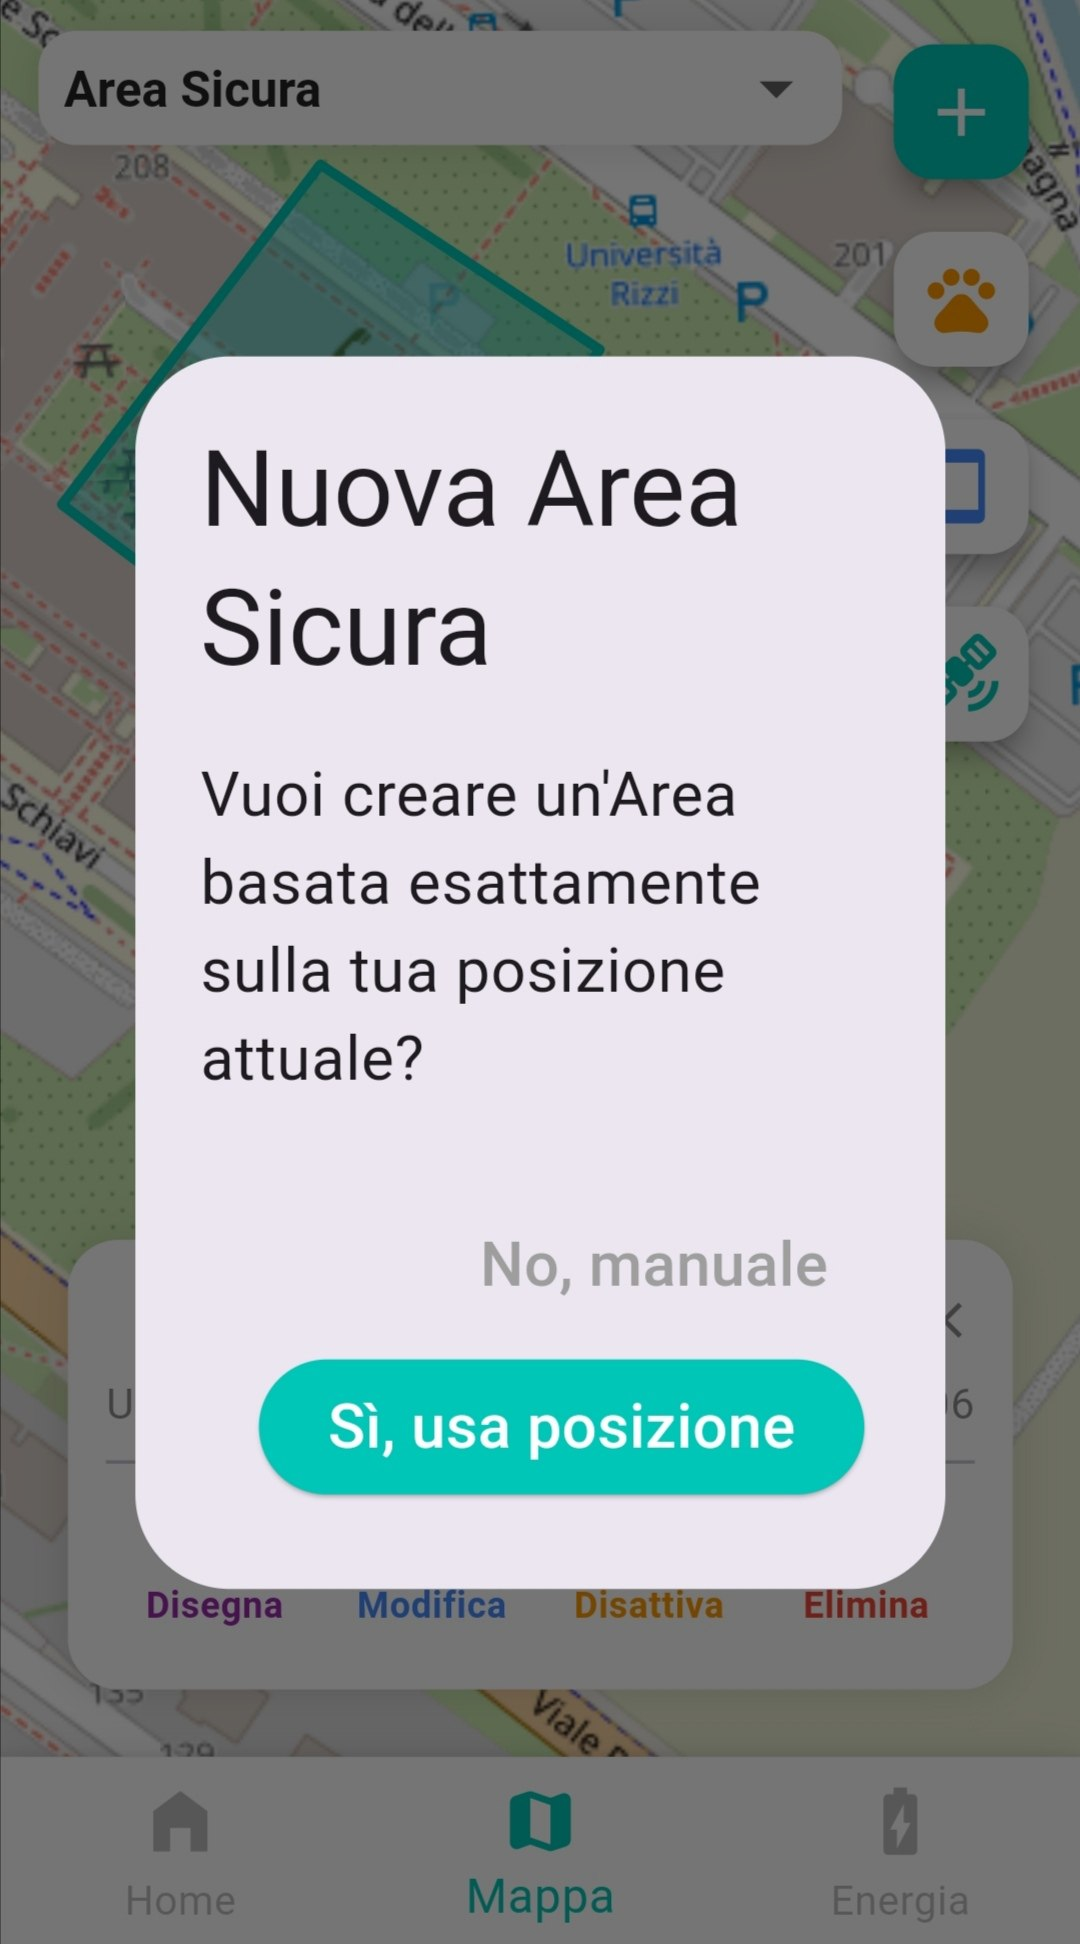
\includegraphics[width=\textwidth, height=8cm, keepaspectratio]{immages/section_5/photo_5.jpg}
        \caption{Scelta dell'inserimento.}
        \label{fig:area_choose}
    \end{subfigure}
    \hfill 
    % Seconda immagine (Centro)
    \begin{subfigure}[b]{0.31\textwidth}
        \centering
        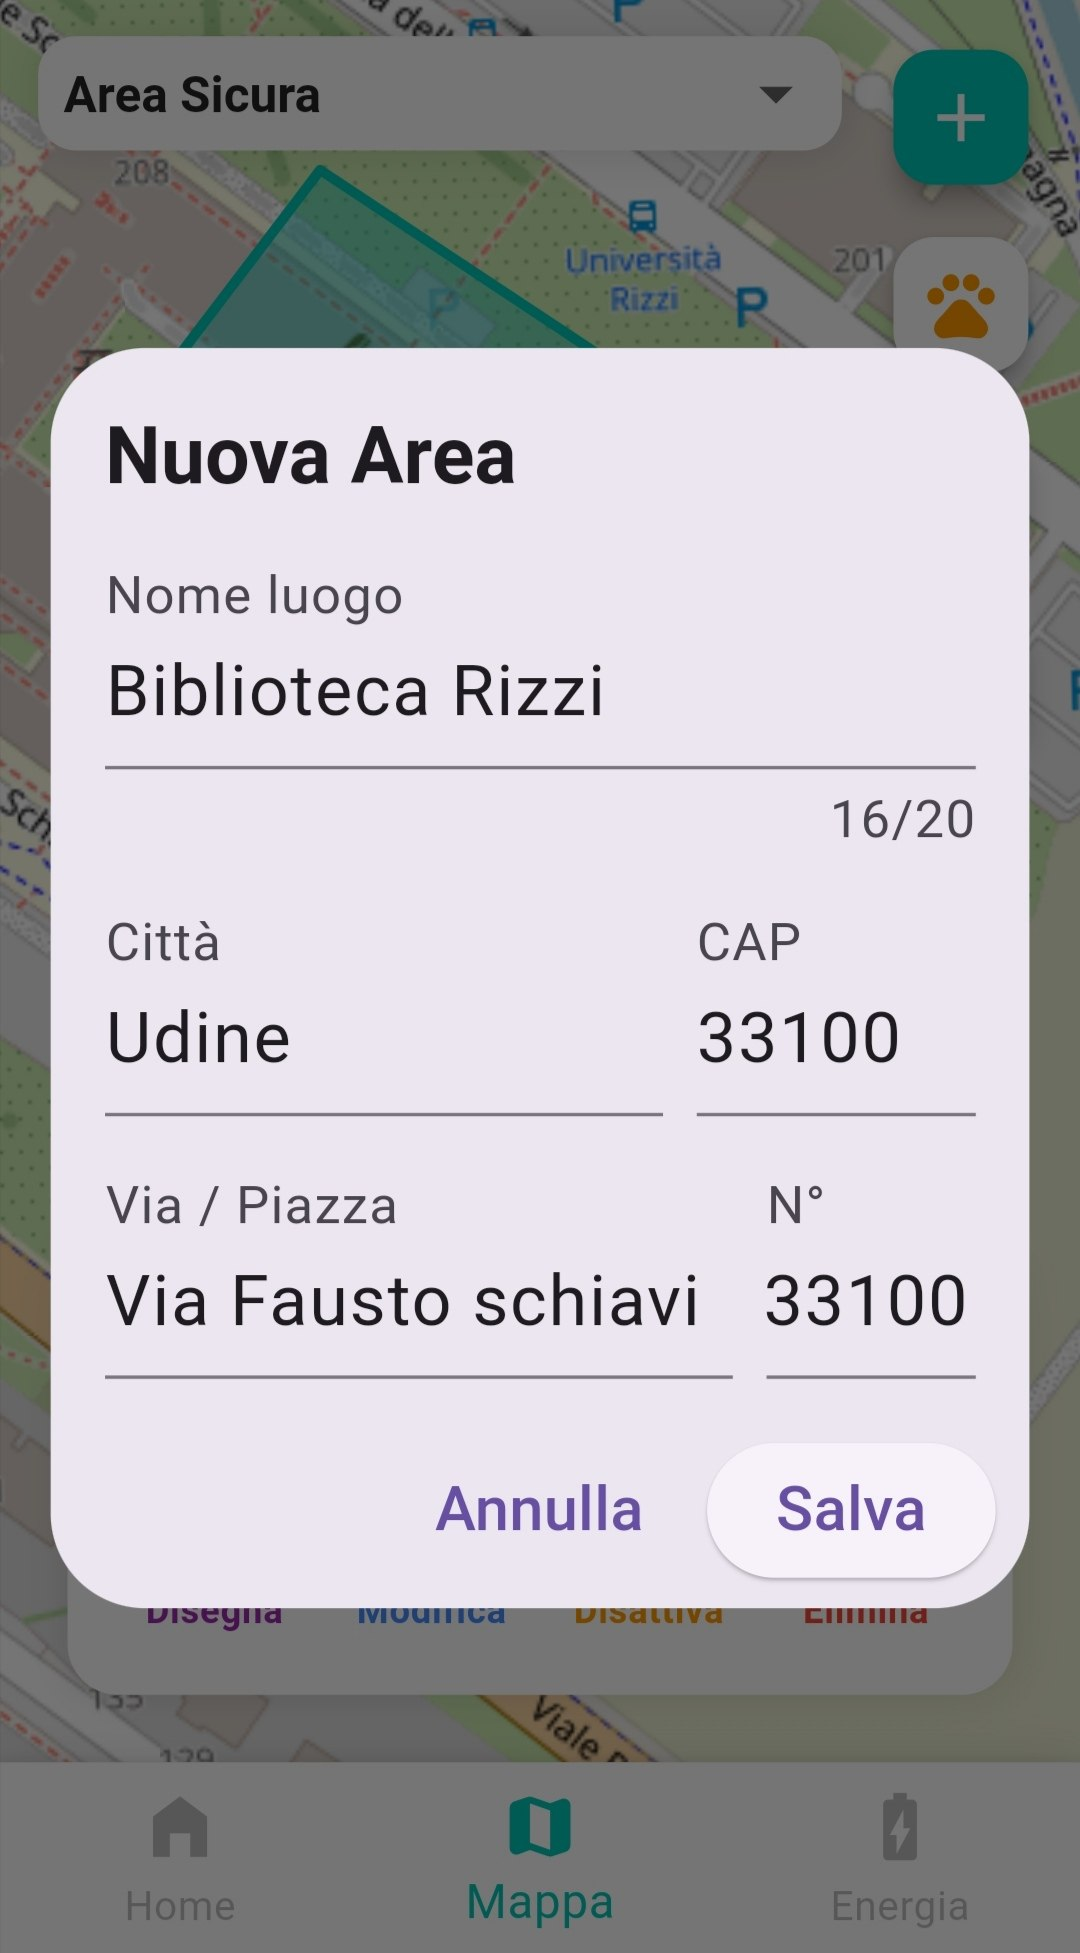
\includegraphics[width=\textwidth, height=8cm, keepaspectratio]{immages/section_5/photo_4.jpg}
        \caption{Compilazione indirizzo.}
        \label{fig:area_form}
    \end{subfigure}
    \hfill 
    % Terza immagine (Destra)
    \begin{subfigure}[b]{0.31\textwidth}
        \centering
        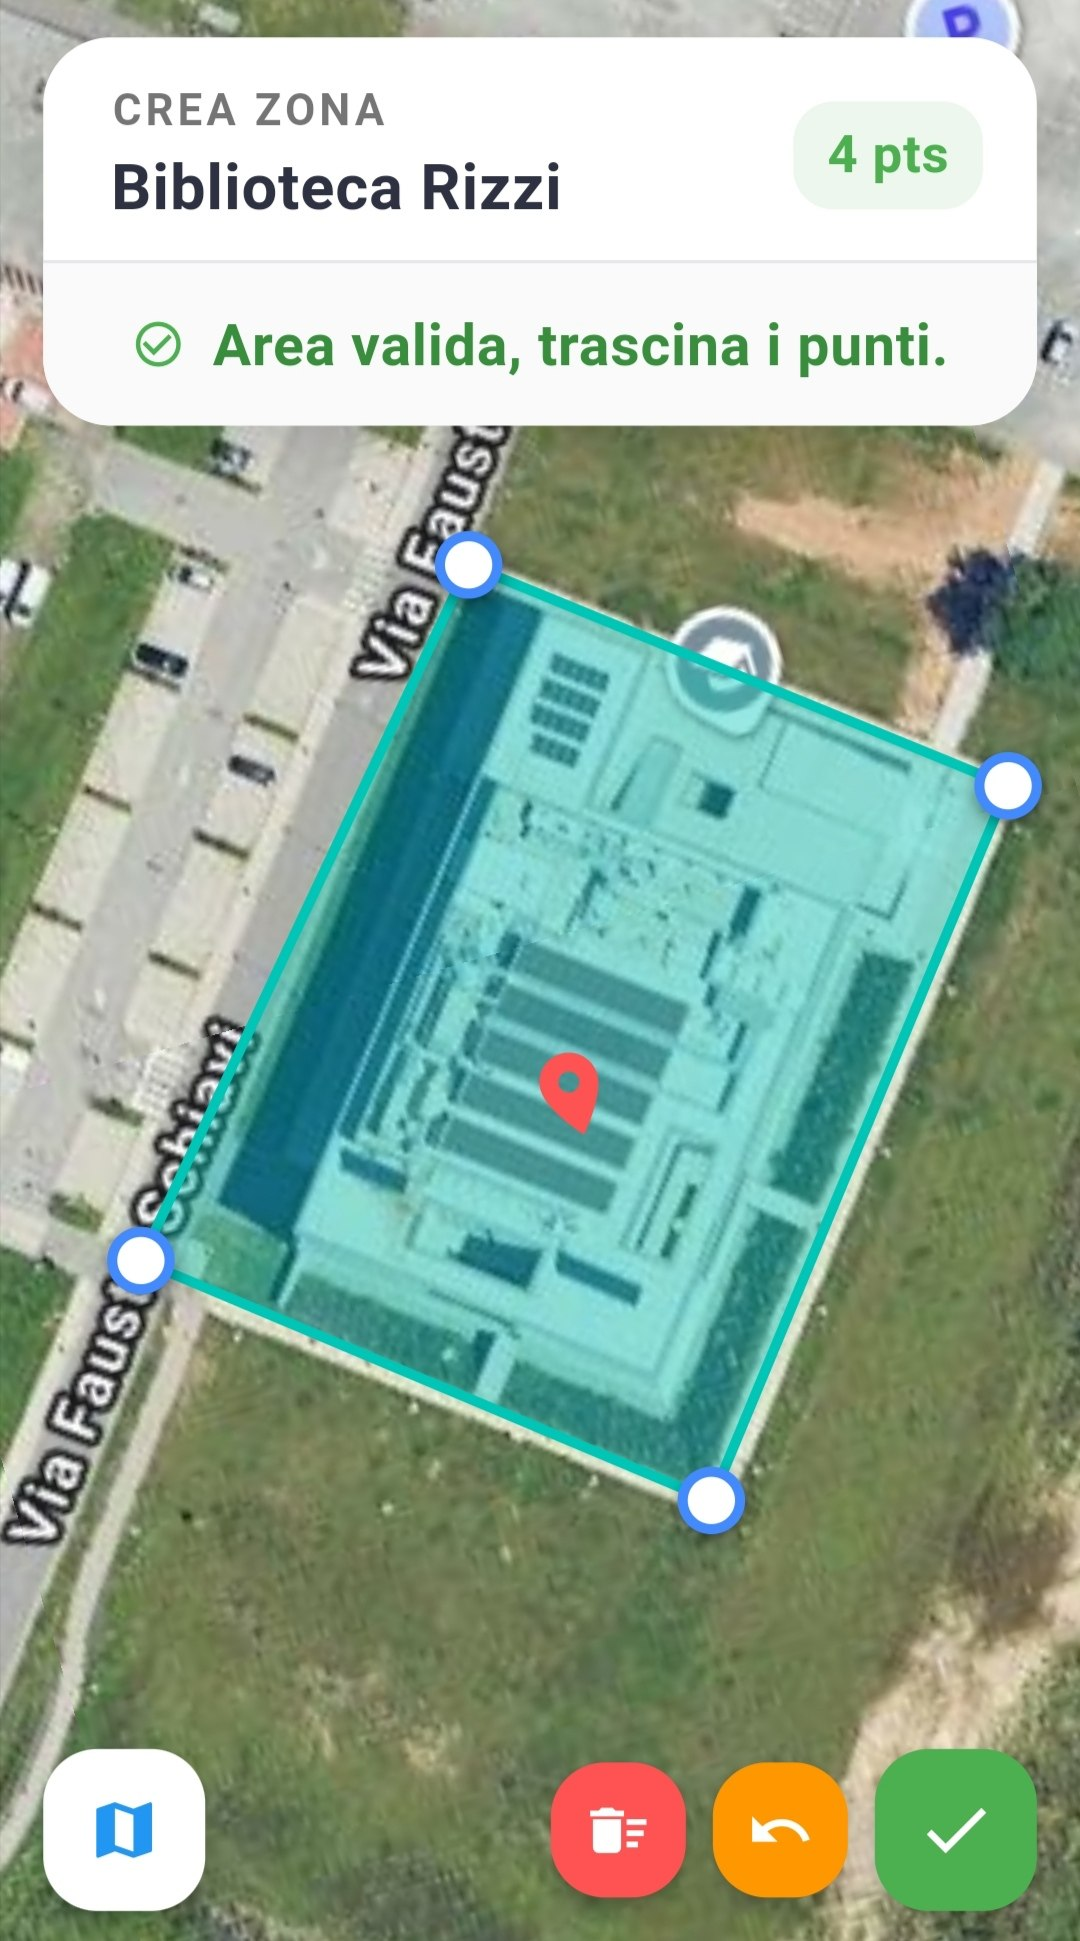
\includegraphics[width=\textwidth, height=8cm, keepaspectratio]{immages/section_5/photo_2.jpg}
        \caption{Disegno dell'area.}
        \label{fig:area_mappa}
    \end{subfigure}
    \label{fig:creazione_area}
\end{figure}

\section{Sistema di notifiche push}
L'implementazione di un sistema di notifiche push è fondamentale per un dispositivo di tracciamento animali, 
in quanto permette di avvisare tempestivamente l'utente in caso di pericoli (uscita dal perimetro sicuro) o problemi tecnici (batteria scarica).

\subsection{Analisi dei vincoli tecnologici}
Durante la fase di sviluppo, è emerso un vincolo tecnico significativo riguardante 
l'integrazione tra il backend PocketBase e l'SDK ufficiale di Firebase. 
PocketBase è scritto in linguaggio \texttt{Go} e utilizza \textbf{Goja} come motore di esecuzione JavaScript 
per la gestione della logica server-side (hooks). 
Goja è un'implementazione di ECMAScript 5.1 che presenta limitazioni strutturali rispetto a un ambiente Node.js \cite{nodejs} standard:
\begin{itemize}
    \item \textbf{Mancanza di moduli nativi}: Goja non supporta i moduli core di Node.js (come \texttt{fs}, \texttt{crypto} o \texttt{net}), indispensabili per il funzionamento dell'SDK di Firebase.
    \item \textbf{Runtime isolato}: l'SDK \texttt{firebase-admin} \cite{firebase_admin} richiede un ambiente di esecuzione completo per gestire l'autenticazione tramite Service Account e le connessioni persistenti ai server Google.
\end{itemize}

Per superare queste limitazioni, è stata adottata un'architettura \textbf{Bridge}, separando la logica applicativa dall'invio fisico dei messaggi.

\subsection{Architettura del FCM Bridge}
Il sistema si basa su un microservizio esterno sviluppato in Node.js \cite{nodejs}, denominato \textit{FCM Bridge}. L'interazione avviene secondo il seguente flusso:
\begin{enumerate}
    \item \textbf{PocketBase (Goja)}: rileva un evento (es. batteria scarica) e invia una richiesta HTTP POST al bridge tramite il modulo interno \texttt{\$http.send}.
    \item \textbf{FCM Bridge (Node.js)}: riceve la richiesta, carica il Service Account di Firebase e inoltra la notifica tramite l'SDK ufficiale \cite{firebase_admin}.
    \item \textbf{Invio notifica}: il bridge restituisce lo stato della consegna. In caso di errore \texttt{404} (token non registrato, app disinstallata) o \texttt{400} (token malformato), il backend provvede alla rimozione automatica del token dal profilo utente. I token FCM sono memorizzati come array JSON per supportare più dispositivi per singolo utente.
\end{enumerate}
\subsection{Logica di invio e trigger}
Le notifiche vengono scatenate dai seguenti eventi, 
ciascuno con logica contestuale per evitare invii ridondanti nella Tabella~\ref{tab:notifiche}.

\begin{table}[H]
\centering
\begin{tabular}{@{}lp{4.5cm}p{5cm}@{}}
\toprule
\textbf{Evento} & \textbf{Condizione di trigger} & \textbf{Nota} \\
\midrule
Uscito dalla zona                 & \texttt{i} $\to$ \texttt{s} oppure \texttt{i} $\to$ \texttt{w} & Dipende dallo stato allarme               \\
Rientro in zona                   & \texttt{s} $\to$ \texttt{i} oppure \texttt{w} $\to$ \texttt{i} & Presenza di geofence                      \\
Allarme in passeggiata            & \texttt{w} $\to$ \texttt{s}                                    & Attivazione allarme                       \\
Inizio viaggio confermato         & qualsiasi $\to$ \texttt{v/r}                                   & Dipende dallo stato allarme               \\
Fine viaggio in zona              & \texttt{v/r} $\to$ \texttt{i}                                  & Rientro in geofence                       \\
Fine viaggio fuori zona           & \texttt{v/r} $\to$ \texttt{s}                                  & Se allarme attivo                         \\
Fine viaggio fuori zona           & \texttt{v/r} $\to$ \texttt{w}                                  & Se allarme spento                         \\
Nessuna geofence                  & \texttt{i} o \texttt{s} $\to$ \texttt{w}                       & Assenza di geofence                       \\
Batteria bassa                    & $\leq 20\%$                                                    & Solo al cambio di soglia                  \\
Batteria critica                  & $\leq 10\%$                                                    & Solo al cambio di soglia                  \\
Batteria in carica                & \texttt{charging} passa a \texttt{true}                        & Solo al cambio di stato                   \\
Watchdog                          & Silenzio $>$ 10 minuti                                         & Chiusura automatica                       \\
\bottomrule
\end{tabular}
\caption{Trigger del sistema di notifiche push}
\label{tab:notifiche}
\end{table}

\newpage

\subsection{Gestione permessi}

Per abilitare la ricezione delle notifiche lato client, 
è stato fondamentale integrare 
il file di configurazione \texttt{google-services.json}, 
generato direttamente dalla console di Firebase 
e inserito all'interno della directory \texttt{android/app} del codice sorgente.
Questo file contiene le chiavi API, l'identificativo del progetto (\texttt{Project ID}) 
e i dettagli di configurazione necessari per autenticare in modo sicuro 
l'applicazione mobile con i servizi Google, 
senza esporre le credenziali nel codice in chiaro. 
Durante la fase di build, il \textit{plugin Gradle} di Google Services,
che si occupa di mappare i parametri di configurazione nel codice Android,
processa questo file per inizializzare automaticamente 
l'SDK di Firebase all'avvio dell'app,
abilitando così la connessione sicura a FCM 
e la generazione del token univoco del dispositivo.
Quest'ultimo viene dapprima salvato localmente 
e poi sincronizzato con il profilo utente su PocketBase 
all'interno del campo \texttt{tokenFCM}. 
Prima di ogni salvataggio, viene effettuato un controllo di duplicazione 
che verifica se il \textit{token} non sia già presente, 
evitando così la ricezione di notifiche ridondanti.

\section{Vincoli di sistema}
Nonostante i risultati ottenuti, il sistema presenta alcune limitazioni:
\begin{itemize}
    \item \textbf{Dipendenza dalla rete LTE}: senza copertura la trasmissione dati non è garantita.
    \item \textbf{Prestazioni indoor}: il modulo GNSS risulta poco affidabile in ambienti chiusi.
    \item \textbf{Backend locale}: l'utilizzo di PocketBase su macchina locale, 
        esposto tramite ngrok, introduce dipendenze da servizi esterni e limita la scalabilità.
    \item \textbf{Race condition sui pacchetti}: in caso di ricezione 
        quasi simultanea di due pacchetti dallo stesso dispositivo, 
        entrambi potrebbero leggere lo stesso record \texttt{activity} 
        prima del completamento della prima scrittura. 
        Gli scenari più critici sono due: 
        \begin{itemize}
            \item Se entrambi i pacchetti rilevano un cambio di stato, 
                il secondo potrebbe sovrascrivere un record già chiuso dal primo, 
                generando inconsistenze strutturali.
            \item Se entrambi i pacchetti riattivano 
                lo stesso record \texttt{sleep}, potrebbero creare due sessioni attive 
                contemporaneamente, violando l'invariante del sistema.
        \end{itemize}
        L'impossibilità di gestire transazioni atomiche 
        sui singoli record tramite le API di PocketBase 
        rende questo scenario non eliminabile lato applicativo. 
        Tuttavia, la frequenza di invio (ogni 30~s circa) 
        rende l’evento estremamente raro nella pratica.
    \item \textbf{Fallimento nella geolocalizzazione}: l'eventuale mancato rilevamento 
        di indirizzi, solitamente nei centri abitati più piccoli, 
        non è imputabile al codice, bensì a un limite legato alla densità dei metadati geografici. 
        Poiché \texttt{OpenStreetMap} si basa su contributi volontari, 
        l'assenza di tag specifici (come i numeri civici o il CAP associato alla via) 
        rende inefficaci le query strutturate inviate a \texttt{Nominatim}. 
        Quest'ultimo, richiedendo una corrispondenza rigida ed esatta di tutti i parametri forniti, 
        non è in grado di compensare l'incompletezza dei dati.
\end{itemize}

\section{Sviluppi futuri e prospettive del progetto}
Durante lo sviluppo sono emerse diverse opportunità di scalabilità del progetto, 
illustrate di seguito tramite alcune proposte di ottimizzazione ed estensione delle funzionalità.

\subsection{Evoluzione e scalabilità del backend}
L'evoluzione dall'attuale prototipo locale a una soluzione più robusta ed efficace richiederà 
la migrazione dell’intero backend su un’infrastruttura Cloud dedicata, 
adottando soluzioni PaaS o VPS (come AWS, Google Cloud o DigitalOcean). 
Questa evoluzione consentirà di superare i vincoli attuali attraverso i seguenti interventi strutturali:
\begin{itemize}
    \item \textbf{Assegnazione di dominio e sicurezza TLS:} sostituendo il tunnel temporaneo \texttt{ngrok} con un dominio di secondo livello proprietario, protetto da certificati SSL/TLS (es. \texttt{Let's Encrypt}), garantirà una connessione HTTPS/WSS, stabile e priva di interruzioni di sessione o limiti di traffico.
    \item \textbf{Risoluzione delle race condition:} per eliminare il rischio di collisioni causato dall'arrivo simultaneo di pacchetti, si prevede l'introduzione di un middleware di messaggistica asincrona, come \texttt{Redis} o \texttt{RabbitMQ}, tra l'endpoint di ricezione e il database. Questo livello fungerà da coda FIFO (\textit{First-In, First-Out}), mettendo in fila i pacchetti provenienti dallo stesso dispositivo per elaborarli rigorosamente uno alla volta, garantendo così la coerenza dei dati nel database.
    \item \textbf{Migrazione del DBMS:} qualora il volume di dispositivi connessi diventasse troppo elevato per le capacità di SQLite, sarà possibile migrare verso un database più robusto (come \texttt{PostgreSQL}), progettato appositamente per gestire un grande volume di scritture simultanee senza bloccarsi.
\end{itemize}

\subsection{Evoluzione e costruzione hardware}
L’attuale prototipo è stato fondamentale per testare il software, ma richiederà un'ottimizzazione dell'hardware per diventare un dispositivo pratico da far indossare all'animale. Lo sviluppo futuro si articolerà su tre assi principali:
\begin{itemize}
    \item \textbf{Sviluppo di un PCB custom:} progettare un'unica scheda su misura (es. \texttt{KiCad}) che integri microcontrollore, modem LTE e modulo GNSS. In questo modo si ridurranno drasticamente le dimensioni e il peso del dispositivo sul collare dell'animale.
    \item \textbf{Ottimizzazione del power management:} l'integrazione di un \textit{PMIC} e di un chip fuel gauge (es. \texttt{MAX17043}) permetterà di ottenere letture della batteria estremamente precise. Questo abiliterà il calcolo predittivo sui dati storici, evitando che i picchi di consumo del modem durante le trasmissioni falsino la percentuale di carica.
    \item \textbf{Design e protezione:} progettazione di un involucro su misura, ad esempio tramite modellazione 3D e stampaggio a iniezione. La scocca dovrà avere una certificazione minima \textbf{IP67} o \textbf{IP68} per garantire totale impermeabilità (ad acqua e fango) e resistere agli urti causati dai movimenti dell'animale.
\end{itemize}

\newpage

\section{Conclusioni}
Il progetto Pet Tracker ha raggiunto l'obiettivo dichiarato in fase di progettazione: realizzare un sistema end-to-end, dal dispositivo embedded indossabile fino all'applicazione mobile, in grado di monitorare in tempo reale la posizione, l'attività motoria e lo stato energetico di un animale domestico, con particolare attenzione alla sicurezza (geofencing e allarme) e all'efficienza energetica del nodo IoT.


Dal punto di vista hardware, l'integrazione su scheda LilyGo T-SIM7670G-S3 tra microcontrollore ESP32-S3, modem LTE, modulo GNSS e accelerometro BMA400 ha dimostrato la fattibilità di un tracker autonomo, mentre le strategie di \textit{deep sleep} e \textit{hot start} hanno permesso di contenere i consumi senza sacrificare la reattività del sistema. 

A livello firmware e backend, la scelta di PocketBase si è rivelata efficace per la rapidità di sviluppo, sebbene abbia introdotto vincoli non banali, primo fra tutti l'incompatibilità del motore Goja con l'SDK di Firebase, risolta tramite l'introduzione di un microservizio \textit{bridge} dedicato. 

Sul fronte applicativo, l'app Flutter ha concretizzato un'architettura visiva a livelli chiara migliorandone l'interfaccia, mentre l'adozione di \path{Server-Sent Events} e l'implementazione locale del geofencing hanno permesso di ottenere un'esperienza utente reattiva e a basso impatto energetico. 

Il sistema di notifiche push, pur richiedendo un'architettura a bridge per aggirare i limiti del runtime server-side, copre in modo puntuale gli eventi rilevanti per l'utente rendendo il prodotto realmente utilizzabile in scenari reali di sorveglianza dell'animale.

Il lavoro svolto non è tuttavia esente da limiti, in parte intrinseci alla fase di prototipazione: la dipendenza da un backend locale esposto tramite ngrok, l'assenza di un meccanismo di transazioni atomiche per la gestione della concorrenza sui pacchetti quasi simultanei e l'affidabilità non uniforme del reverse geocoding basato su OpenStreetMap rappresentano i principali fattori di rischio per una messa in produzione su larga scala. 

Si tratta, in ogni caso, di limitazioni ben circoscritte e già indirizzate concettualmente nel capitolo dedicato agli sviluppi futuri.

In sintesi, il progetto dimostra concretamente come i principi dell'IoT (acquisizione edge, trasmissione a basso consumo, elaborazione server-side e restituzione di dati già astratti al client) possano essere applicati con successo a un caso d'uso reale e di forte valore pratico, ponendo al contempo basi solide e ben documentate per un'evoluzione futura verso un sistema scalabile e production-ready.

\clearpage
\addcontentsline{toc}{section}{Riferimenti bibliografici}
\printbibliography[title={Riferimenti bibliografici}]

\end{document}